\documentclass[conference]{IEEEtran}
\IEEEoverridecommandlockouts

\usepackage{cite}
\usepackage{amsmath,amssymb,amsfonts}
\usepackage{algorithmic}
\usepackage{graphicx}
\usepackage{textcomp}
\usepackage{float}
\usepackage{xcolor}
\usepackage[a4paper, total={184mm,239mm}]{geometry}
\def\BibTeX{{\rm B\kern-.05em{\sc i\kern-.025em b}\kern-.08em
    T\kern-.1667em\lower.7ex\hbox{E}\kern-.125emX}}

\usepackage{listings}
\usepackage{booktabs}
\usepackage{multirow}
\usepackage[normalem]{ulem}
\useunder{\uline}{\ul}{}
\usepackage{url}
\usepackage{fancyvrb}

\lstdefinestyle{Scalastyle}{
    language=scala,
    aboveskip=3mm,
    belowskip=3mm,
    showstringspaces=false,
    columns=flexible,
    basicstyle={\small\ttfamily},
    numberstyle=\tiny\color{gray},
    keywordstyle=\color{blue},
    commentstyle=\color{dkgreen},
    stringstyle=\color{mauve},
    breaklines=true,https://www.overleaf.com/project/63bd7510cad851deec6a46dc
    breakatwhitespace=true,
    tabsize=2,
    numbers=left,
    xleftmargin=2em,
    frame=single,
    framexleftmargin=1.5em,
    captionpos=b
}

\definecolor{mGreen}{rgb}{0,0.6,0}
\definecolor{mGray}{rgb}{0.5,0.5,0.5}
\definecolor{mPurple}{rgb}{0.58,0,0.82}
\definecolor{backgroundColour}{rgb}{0.95,0.95,0.92}

\lstdefinestyle{Cstyle}{
    language=C,
    aboveskip=3mm,
    belowskip=3mm,
    showstringspaces=false,
    columns=flexible,
    basicstyle={\small\ttfamily},
    numberstyle=\tiny\color{gray},
    keywordstyle=\color{blue},
    commentstyle=\color{mGreen},
    stringstyle=\color{mPurple},
    breaklines=true,
    breakatwhitespace=true,
    tabsize=2,
    numbers=left,
    xleftmargin=2em,
    frame=single,
    framexleftmargin=1.5em,
    captionpos=b
}

\begin{document}

\title{Parallelization of genetic algorithm}

\author{
    \IEEEauthorblockN{Bruno Perković}
    \IEEEauthorblockA{
        \textit{University of Zagreb, FER} \\
        \textit{Zagreb, Croatia}\\
        bruno.perkovic@fer.hr
    }
    \and
    \IEEEauthorblockN{Darijan Gudelj}
    \IEEEauthorblockA{
    \textit{University of Zagreb, FER} \\
        \textit{Zagreb, Croatia}\\
        darijan.gudelj@fer.hr
    }
}


\maketitle

\begin{abstract}
     This paper describes a method for training a neural network to control the movement of a character in a walking simulation using GLSL and an evolutionary algorithm for a realistic and efficient motion.
\end{abstract}

\begin{IEEEkeywords}
    GLSL, OpenGL, genetic algorithm, neural network, physics simulation, Pytorch
\end{IEEEkeywords}

%We want to lower costs with energy efficiency as well
\section{\huge Introduction}
        In this paper, we present a method for training a neural network to control the movement of a character in a custom physics simulation of walking using GLSL. Our approach utilizes an evolutionary algorithm to optimize the network's parameters, with the goal of achieving a realistic and efficient walking motion. The custom physics simulation is designed to be highly parallelizable, which allows for real-time interactive control of the character's movement. We also show how Pytorch was used as an experimentation tool before building the final implementation in GLSL.
    
\section{\huge Background}
    \subsection{\Large Pytorch and Python}
    \textbf{Pytorch}\cite{Stevens} is an open-source machine learning library based on the Torch library. It was developed by Facebook's artificial intelligence research group and was released in 2016. PyTorch is commonly used for applications such as natural language processing and computer vision. It offers a dynamic computational graph, a feature that allows for more flexibility and ease of use when building and training neural networks. Additionally, PyTorch includes support for CUDA, a parallel computing platform and API for GPU-accelerated computing, making it well-suited for training large, deep neural networks on powerful hardware. It has become a popular library in the research community, largely due to its dynamic computation graph and built-in support for CUDA. While primarily developed for GPU, Pytorch enables running the computations on CPU also. In this work we use it to enable fast prototyping and CPU benchmarking.

    \textbf{Python}. PyTorch is a library built for Python. One of the key features of PyTorch is its ability to enable fast iteration times and easy debugging. With PyTorch, developers can easily perform complex operations on tensors (multidimensional arrays) without the need for explicit computation graphs. Additionally, PyTorch's built-in debugging tools, such as the ability to track gradients and perform dynamic graph visualization, make it easier to identify and correct errors in the model. This makes PyTorch a popular choice for researchers and practitioners.

     Both \textbf{Numpy} and PyTorch are powerful libraries for handling multidimensional arrays and performing mathematical operations on them. However, in our application, we chose to use PyTorch because of its native support for neural network operations. In particular, PyTorch provides a convenient module called nn, which includes a wide range of commonly used neural network layers, such as nn.ReLU, that make it easy to build and train complex models. This is the reason we choose Pytorch over Numpy
    \subsection{\Large OpenGL and GLSL}
    \textbf{OpenGL}\cite{Sellers}\cite{Vries} is a cross-platform graphics API that is widely used for developing interactive 2D and 3D applications. It is a powerful and flexible tool that allows programmers to create rich visual experiences by drawing and manipulating 3D objects, textures, and lighting in a 3D environment. OpenGL is supported by a wide range of hardware and software platforms, including desktop and mobile devices, game consoles, and web browsers.

    \textbf{GLSL} (OpenGL Shading Language) is the programming language used to create shaders in OpenGL. Shaders are small programs that are executed on the graphics processing unit (GPU) and allow developers to write custom code to control the way that 3D objects are rendered. GLSL provides a wide range of built-in functions and data types that can be used to create a wide variety of effects, from simple per-pixel lighting to more advanced features such as depth of field, reflections, and more.
    
    In scientific applications, OpenGL and GLSL can be used to create interactive visualizations of complex data sets, such as simulations of physical phenomena, medical imaging, and more. The GPU's parallel processing capabilities allow for real-time interaction and manipulation of large data sets, which can be useful in fields such as data analysis, scientific research and discovery, and even interactive training simulations.
    
    One of the many advantages of using GLSL is the flexibility it provides in customizing and optimizing the pipeline of data, allowing the scientist to perform complex mathematical operation in the graphics pipeline, while being able to visualize the outcome in real time.
    
    In summary, OpenGL and GLSL are powerful tools that can be used in scientific applications to create interactive and visually rich visualizations of complex data sets. They allow scientists to analyze and manipulate data in real-time, making it a valuable addition to the scientific toolset.

    \textbf{Compute Shaders} are a specific type of shader that were introduced in OpenGL 4.3 and later. They are designed to perform general-purpose computation on the GPU, as opposed to the traditional rasterization-based pipeline used for rendering graphics. Compute shaders are executed on the GPU's stream processors, which are highly parallel units that can perform many calculations simultaneously.

    Compute shaders are written in GLSL and are executed on a three-dimensional grid of thread groups, each consisting of a fixed number of threads. The programmer defines the layout of the grid and the number of threads per group, and the GPU schedules the execution of the threads. The programmer can synchronize and communicate between different thread groups and between threads within the same group.

    % 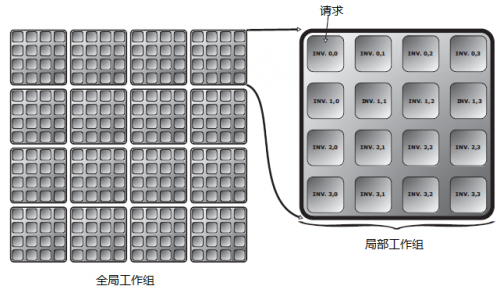
\includegraphics[width=3in]{resources/Compute.jpg}
    
    One of the advantages of using compute shaders is their ability to perform large amounts of data-parallel computation on the GPU. This can be much faster than performing the same computation on the CPU, especially for problems that can be easily parallelized. Additionally, compute shaders can also access memory resources such as textures and buffer objects, allowing the programmer to manipulate and store large data sets directly on the GPU.

\section{\huge Main}
     \subsection{\LARGE Experimentation}
\subsubsection{\textbf{\large Physics engine}}
    We model every body as a collection of points. The points interact with each other through spring forces, two points interact if they are connected via a spring, there is no collision detection between points. This all means that there is no inherent difference between a bone or a muscle in a creature, they are both modeled as springs, while they can have different spring coefficients, we found that there are not that many stable configurations of those parameters. Each spring is also damped, damping level is controlled by a special parameter. As with the different spring coefficients we found random damping coefficients also unstable. The engine also features gravity force and ground force, both of those forces work on individual points. If one point is acted upon by the ground force the force is carried around through the whole body via spring forces.
    Ground force is modeled by a linearly rising force that starts rising from 0 after the point crosses the "ground line". Ground force also has a damping coefficient.

\subsubsection{\textbf{\large Neural networks}}
    The points of the creature do not and cannot move themselves, we need a learnable controller for creatures to learn to walk.
    While there exist many options, such as learning a program, a decision tree, logistic regression, etc. we decided to use neural networks because of their expresivity. So in this work one neural network controls one creature. It can be thought of as a brain of the creature, and every creature has a different brain. Important thing to point out is that the neural network is the one being optimized by the genetic algorithm. That is the body of the creature is not changing in any way during the evolution. The thing that is changing is its responses which are learned by the neural network. The neural network controls the body by contracting its muscles, the only distinction between muscles and bones is that muscles don't have a constant rest length and bones do. This rest length is controlled with the neural network. Several implementation details and tricks needed to get it to work with satisfactory performance.
        
        \begin{itemize}
            \item \textbf{Neural Network Initialization}

            Linear layers of the neural network are initialized with the He initialization described in Delving deep into rectifiers: "Surpassing human-level performance on ImageNet classification - He, K. et al. (2015), using a uniform distribution". Gain in set at \(\sqrt{2}\) because of the use of Relu (Rectified linear unit) as an activation function. 
            

            \item \textbf{Architecture}

            The neural network has 2 hidden layers of size 32. This means that every network has 3 matrices worth of parameters and 3 vectors. Activation function used in the hidden layers is Relu. Output layer's activation function is the identity.    
            

            \item \textbf{Muscle clamping}

            We did not use muscle clamping in our first experiments which our creatures quickly used to their advantage. Having one point on the ground and moving the muscle to infinity was a winning strategy. This is why we introduced muscle clamping, the muscle can extend or contract only by a certain amount.

            \item \textbf{Relative coordinates}

            While the first version worked, the creatures were learning really slowly, intuitively this is because as they move they have two options, their inputs do not look similar to the ones several steps before. The first option is to learn the new mapping, to convert the coordinates that are now shifted by several steps to actions. The second option is to learn to map the absolute coordinates to local coordinates, which means that when they learn walking in local coordinates they can easily generalize if the input coordinates are shifted. The problem with the second approach is that the conversion should take considerable neural net resources and it will probably make it less fit in the short run, which means it will die and not progress to the next generation. This all means that the creature is stuck in local minima, it cannot go to local coordinates because the evolutionary barrier is to high. This is why we decided to try and in the end use local coordinates. To preserve the neural nets ability to use absolute we added absolute coordinates of the first point. So the input to the neural network are coordinates of the points in the reference frame of the first point and coordinates of the first point in global coordinate frame.

            \item \textbf{Neural net predicts muscle offsets}

            Using the reasoning similar to the one that got us to relative coordinates we changed the output of the network to predict global offsets of the default muscle lengths. If the neural network predicts the offsets relative to the previous frame that would mean that if the neural network changes something in the beginning of the trajectory that that would influence greatly output later in the trajectory. Making neural network predict offsets from the default muscle lengths makes the problem easier to learn and problem parts more independent.
            
        \end{itemize}

    \hfill

\subsubsection{\textbf{\large Genetic algorithm}}
    While there are many different genetic algorithms to choose from, we decided to use the simplest. We select top p percent of creatures to duplicate and bottom b percent to murder. In our experiments we used p=30 and b=50. To give diversity we tried mutating them all, but that did not work well. We found creatures learned more and faster if we kept top k percent of creatures unchanged, we used k=10. The mutation is done by adding a gaussian noise with mean at 0 to the creature's parameters. We fount the exact standard deviation parameter fairly robust and used 1 in our experiments.
    
    
    
    
    \subsection{\LARGE Tools and Dependencies}

    Before we get to implementation of project, we will talk about development environment, tools and libraries we used.

    \subsubsection{\textbf{\large Visual studio 2022}}

        Microsoft IDE which makes handling and debugging multiple complex projects much easier.

    \subsubsection{\textbf{\large Premake}}

        Open source tool for generating cross platform build files for Visual Studio

    \subsubsection{\textbf{\large Tigraf Engine}}

        Graphics Engine which we will use as core of a whole project. From visualisation to speeding up learning algorithms.

\subsection{\LARGE Classes and Initialization}

    \subsubsection{\textbf{\large AppLayer}}

        The Tigraf Engine core operates by sending events, updates, and other actions through layers. In this project, only one layer is required, referred to as the AppLayer. This layer includes the declaration of the necessary functions for the project:

        \hfill
        
        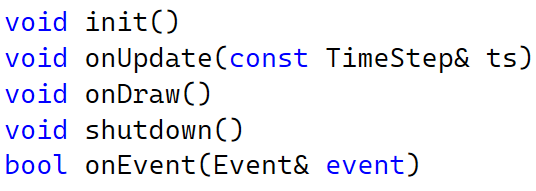
\includegraphics[width=3in]{resources/Layer.png}

        \begin{itemize}
        
            \item \textbf{init}

            Objects are instantiated here and shaders are loaded from memory.

            \item \textbf{onUpdate}

            Here we update the necessary objects and data structures. Most important things here are physics simulation step and neural network which updates movement.

            \item \textbf{onDraw}

            Rendering commands are called from this function. It is used for rendering background, grid and loaded shapes.

            \item \textbf{onEvent}

            All operating system, window and user events are handled here.

            \item \textbf{shutdown}

            This function is mainly used to free memory.
            
        \end{itemize}

    \hfill
    
    \subsubsection{\textbf{\large Shape}}

        This structure defines a look of an entity which is learning how to walk.

        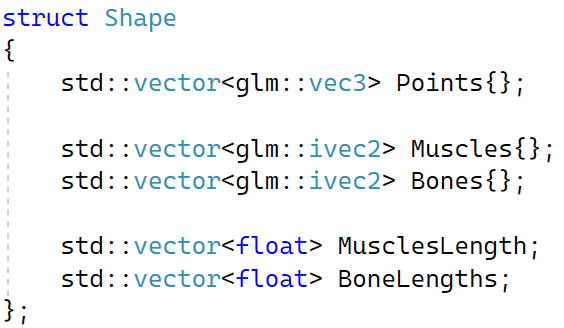
\includegraphics[width=3in]{resources/Shape.png}

    \hfill

    \subsubsection{\textbf{\large ShapeLoader}}

        This class comprises static methods for loading the shape from memory. The points are stored as "points" where each line of text represents a point, with the coordinates separated by spaces. Similarly, there are sections for "bones" and "muscles" where each line of text contains two indices.

    \hfill

    \subsubsection{\textbf{\large ShapeRenderer}}

        This class serves as the main location for methods related to initializing and transferring all required project data to the GPU. The ShapeRenderer class offers a range of static methods for handling tasks such as rendering, simulation, and learning. These methods are called from the AppLayer.

\subsection{\LARGE A closer look into the ShapeRenderer}

        The engine core of the program provides various data structures, including buffers, for the ShapeRenderer to utilize in order to transfer data to the GPU. As the primary objective of this project is to optimize performance, a majority of the buffers employed are RWBuffers, which are enabled for both reading and writing on the GPU side. This approach eliminates the need to constantly copy data to the CPU, thus removing the largest bottleneck in the system. The buffers utilized in this program are listed below for reference.

        \begin{itemize}
            
            \item{\textbf{PosVelBuffer}}
                is used to store positions and velocities of each point for each instance.
                It is modifiable by shaders.

                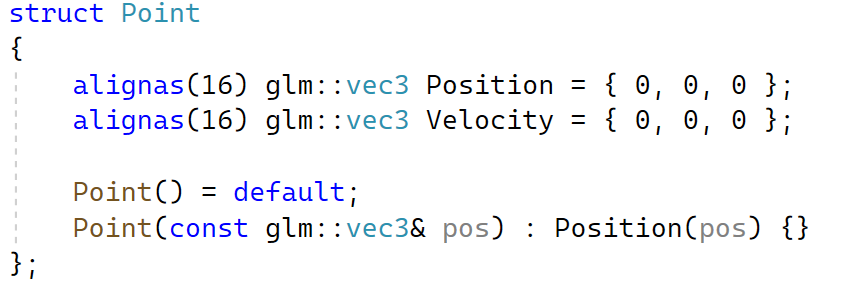
\includegraphics[width=3in]{resources/Point.png}

            \item{\textbf{LengthBuffer}}
                is used to store muscle lengths for each instance.
                It is modifiable by shaders.

            \item{\textbf{LayerBuffer}}
                is used to store 3-layered neural network for each instance. It is filled randomly and it is also modifiable by shaders. The second largest performance bottleneck in the system is identified within this buffer. During the process of instantiating the next generation, the GPU threads require access to data from one another, which necessitates the use of coherency and barrier bits. To address this issue, a solution was implemented by duplicating the buffer and utilizing both copies in a zig-zag fashion. This approach eliminated the need for synchronization throughout the entire project, resulting in a significant improvement in performance!

            \item{\textbf{StatsBuffer}}
                is used for storing statistic data such as instance count, movement distance, mean and variance.
                It is modifiable by shaders.

            \item{\textbf{FitnessIndicesBuffer}}
                is used for storing the fitness of each instance each episode.
                It is modifiable by shaders.

                \item{\textbf{ShapeDataBuffer}}
                is used to store immutable information of shape such as points count, muscles count, default muscle and bone lengths.
                It is a read-only buffer.

                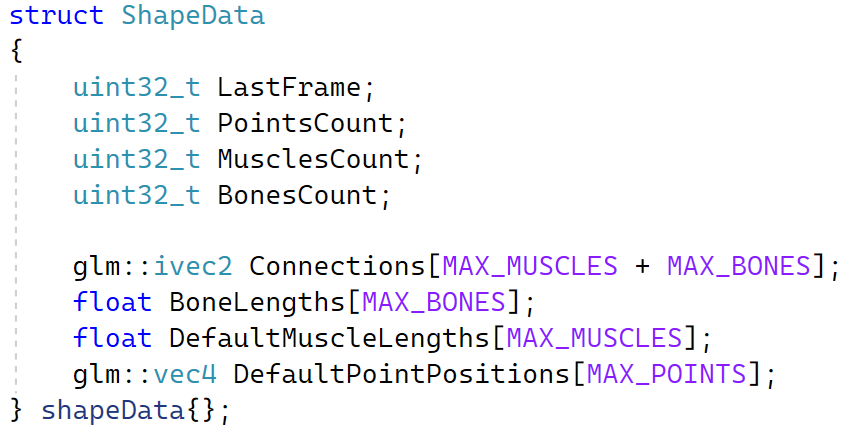
\includegraphics[width=3in]{resources/ShapeData.png}

            \item{\textbf{ShapeVertexBuffer}}
                will be used for storing pairs of indices which form connection and a boolean value saying whether it is a muscle or a bone.
                It is immutable and it will be used for drawing.
                
        \end{itemize}

        \hfill

\subsection{\LARGE Examining the Shaders}

        Apart from initializing buffers, we few compute shaders are also loaded into a memory:

    \subsubsection{\textbf{\large ShapeShader}}
        Used for drawing certain amount of instances. It uses points and connections from \textbf{ShapeVertexBuffer} and \textbf{ShapeDataBuffer} to visualize shape. 
        Depending on the instance id, it connects certain points. With help of normals, tangents and bitangents it creates cuboid limbs and adds lighting effect to each surface.

    \subsubsection{\textbf{\large PhysicsCompute}}
        Used for doing a physics step. It modifies \textbf{PosVelBuffer}.
        Takes previous positions and velocities and modifies them using gravity, damping, springs, friction and floor force. Additionally, it fills \textbf{FitnessIndicesBuffer} on the last iteration of current generation.

    \subsubsection{\textbf{\large GeneticCompute}}
        Used for controlling muscle and shape movement. It modifies the \textbf{LengthsBuffer} by reading the \textbf{LayerBuffer}. It runs through a neural network for each instance with the input of absolute position of the first point, absolute velocity of the first point, all positions relative to the first point and all velocities relative to the first point. The output is new muscle lengths for that instance.

        Output will be new muscle lengths for that instance.

    \subsubsection{\textbf{\large EvolutionCompute}}
        Used for rewarding and reproducing fit instances and, of course, \textbf{murdering} bad instances. It modifies \textbf{LayerBuffer} based on \textbf{FitnessIndicesBuffer}.

\section{\huge Evaluation}

\subsection{\LARGE Exploring the Hardware Limitations}

Before showing project results and benefits of parallel execution, we will take a look on limits we encountered. 

\subsubsection{\textbf{\large CPU limitations}}

\begin{itemize}
    \item The process of sequentially learning and simulating physics on a CPU has been found to be quite slow, particularly when dealing with a relatively high number of instances. Specifically, it has been observed that at around 300 instances, a single iteration \footnote{In this paper, iterations and frames are used interchangeably and each frame corresponds to a single learning and simulation step along with a visual output. Paper also mentions a real-time learning, which here corresponds to approximately 25 frames per second. Although 25 frames per second may not be ideal for interactive applications, it is worth noting that movies are typically shot at 24 frames per second and still appear smooth to viewers. However, we will still aim to present the examples at about 60 frames per second.} of the simulation takes approximately one second to complete. Given that an episode typically lasts between 200 and 400 iterations, this would mean that it would take approximately one hour to complete 10 generations of the simulation. This presents a significant challenge in terms of computational efficiency and highlights the need for more powerful and efficient hardware to effectively handle larger datasets and more complex simulations and that is where the GPU comes.
\end{itemize}

\subsubsection{\textbf{\large GPU limitations}}

\begin{itemize}
    \item The \textbf{visualization} component of the algorithm was able to sustain the rendering of approximately 4 million instances at a rate of 60 iterations per second. The primary requirement for this step was the PosVelBuffer, which consumed a total memory of 1.2-1.5GB on the GPU. The ShapeShader, which is responsible for generating additional 3D coordinates for each connection, further expanded this memory requirement to 4.5-5.0GB. Despite the GPU having a total memory of 6GB, the inclusion of other data such as textures for display resulted in a near-limit usage of memory, which ultimately resulted in a drastic decrease in performance if we were to increase the instance count any further.

    \item The integration of the \textbf{simulation} component with visualization resulted in a noticeable decrease in performance compared to visualization alone. The algorithm was only able to sustain the rendering of approximately 1 million instances at a rate of 60 iterations per second. Despite the inclusion of additional buffers, none were able to match the memory requirement of the PosVelBuffer. Though the reduction in the number of instances resulted in a decrease in memory usage by about 75\%, the addition of physics algorithms and dense computations significantly slowed down the overall performance of the algorithm.

    \item The integration of the \textbf{learning} component with simulation and visualization proved to be the most challenging aspect of the algorithm testing. Each instance required its own neural network, represented by a 3-layered structure. The total matrix size for this component was staggering, with 6000 floats per instance. This represented a significant increase in memory requirements, with a 2 orders of magnitude increase from the previous memory requirements for visualization and simulation alone. This resulted in a return of the previous memory bottleneck, compounded by the intense nature of matrix multiplication and the simultaneous access of a large number of threads to the main memory. As a result, the algorithm was only able to sustain the rendering of 50,000 instances at the end of the testing with 60 iteration per second.

    \begin{figure}[hbt!]
        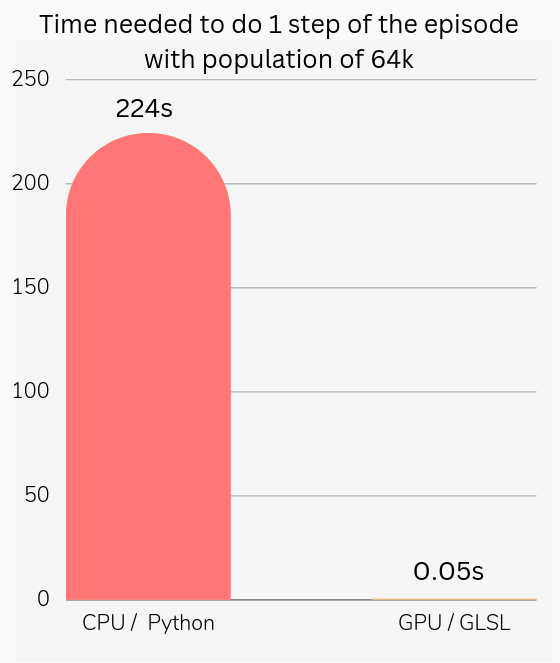
\includegraphics[width=3in]{time1step.png} %veličina u odnosu na širinu linije
        \caption{Illustration of advantage of using GPU's to simulate physics and run creature learning.}
        \label{fig:struktura} %label mora biti drugaciji za svaku sliku
    \end{figure}

    \begin{figure}[hbt!]
        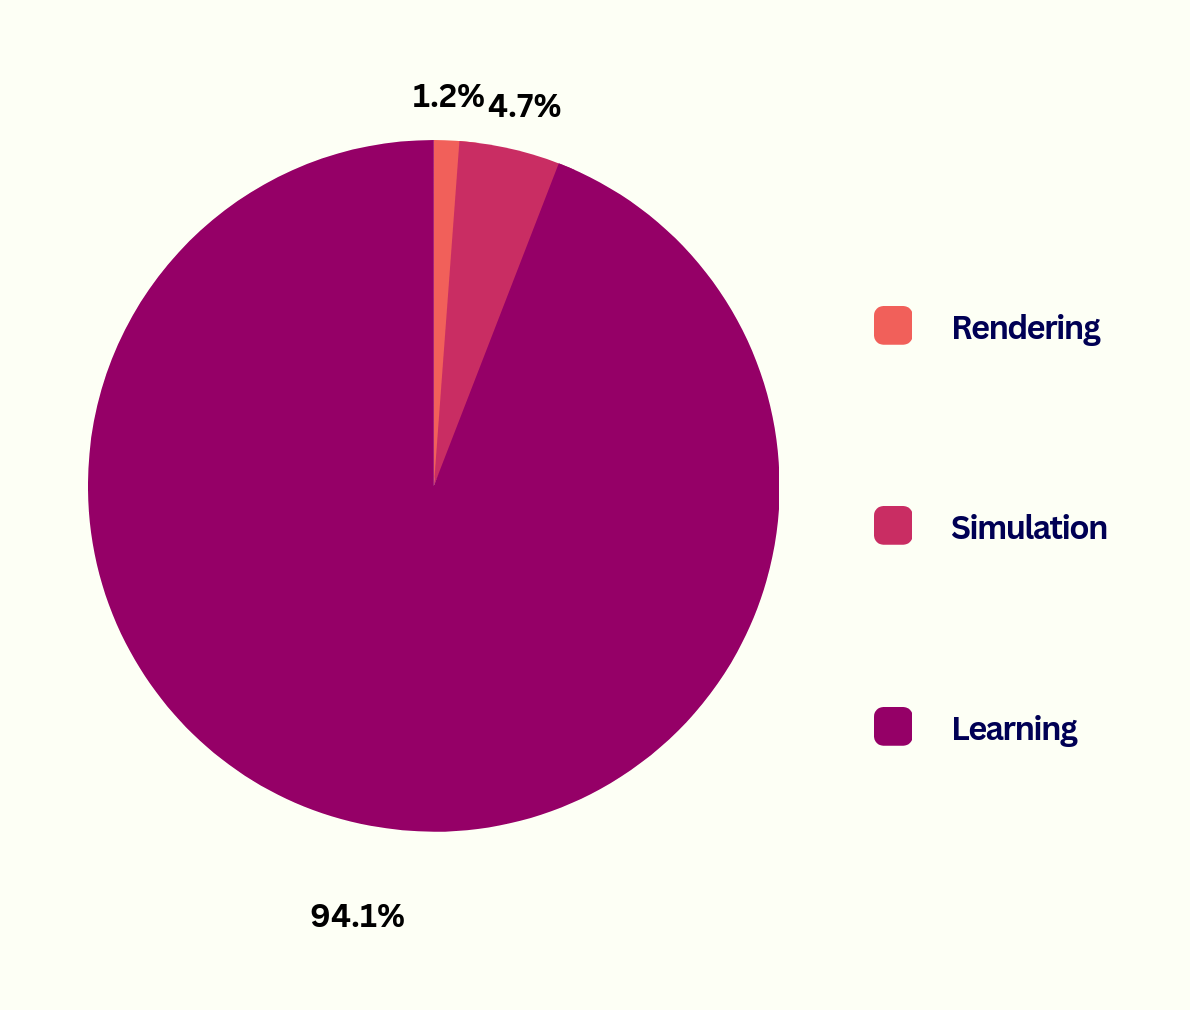
\includegraphics[width=3in]{resources/amdalh.png} %veličina u odnosu na širinu linije
        \caption{An illustration of Amdahl's law in practice. While we could have focused on improving the rendering or simulation the bulk of the time was spent on multiplying matrices, so we decided to leave rendering and simulation and focus on improving learning.}
        \label{fig:struktura} %label mora biti drugaciji za svaku sliku
    \end{figure}
        
\end{itemize}

% \clearpage

\subsection{\LARGE Unveiling the Results}


The next few figures showcase the different performances we get when we employ the CPU or the GPU for our task. \\


Figure 3. illustrates the efficiency of using a GPU to run simulations and evolution, as the GPU time per episode step is much less than the CPU time for larger population sizes. This highlights the advantage of using specialized hardware like a GPU for these types of computationally intensive tasks. \\


Figure 4. showcases the relationship between population size and the number of generations needed for creatures to learn to walk. As the population size increases, the probability that any creature will learn to walk by chance rises. This result suggests that a larger population size can lead to faster convergence and better performance in evolutionary algorithms. \\


\begin{figure}[H]
    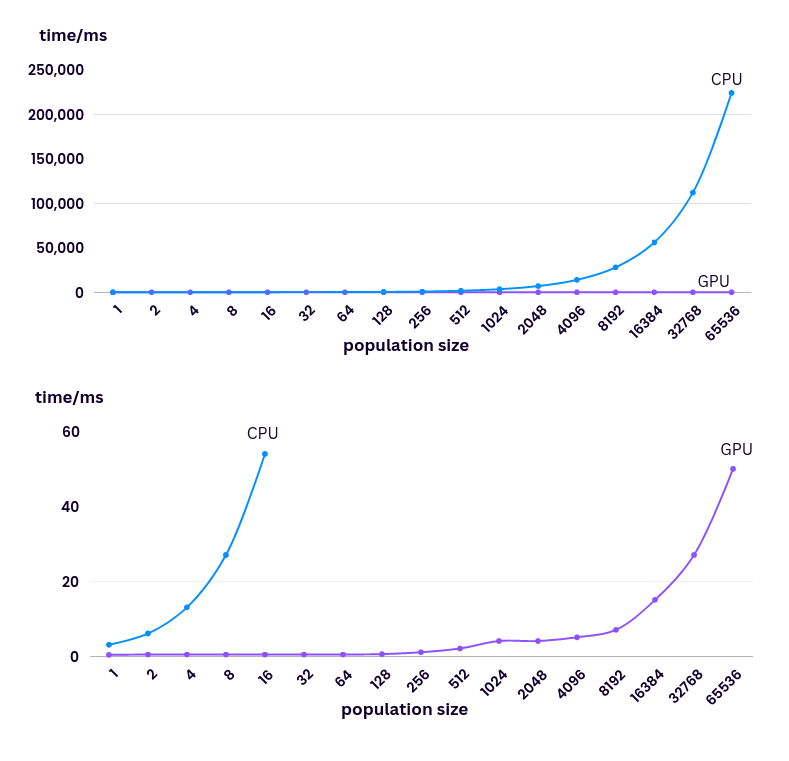
\includegraphics[width=3in]{popsizetime.png} %veličina u odnosu na širinu linije
    \caption{GPU vs CPU time per 1 episode step for different population sizes. GPU is running a program written in GLSL and CPU in Python. It can be seen that the CPU time grows much more quickly.}
    \label{fig:struktura} %label mora biti drugaciji za svaku sliku
\end{figure}

\begin{figure}[H]
    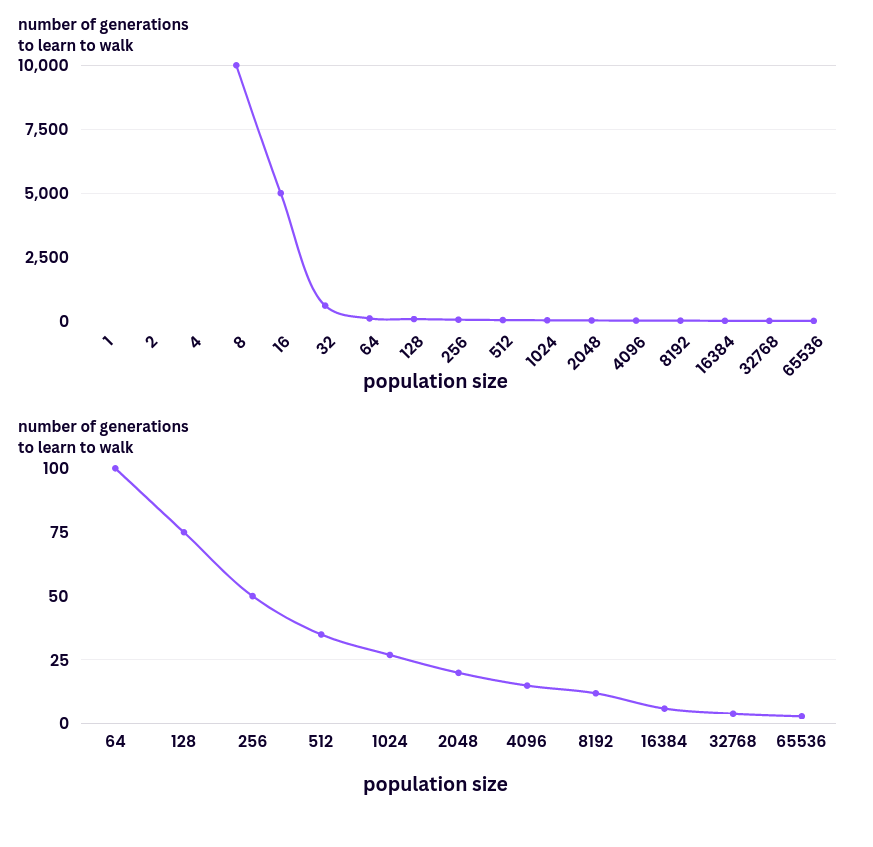
\includegraphics[width=3in]{numberofgenerationstolearntowalk.png} %veličina u odnosu na širinu linije
    \caption{As the population size grows number of generations to learn to walk falls. This is because when the population size is large, the probability that any creature is walking by pure chance is high.}
    \label{fig:struktura} %label mora biti drugaciji za svaku sliku
\end{figure}




%\section{\huge Results}

%
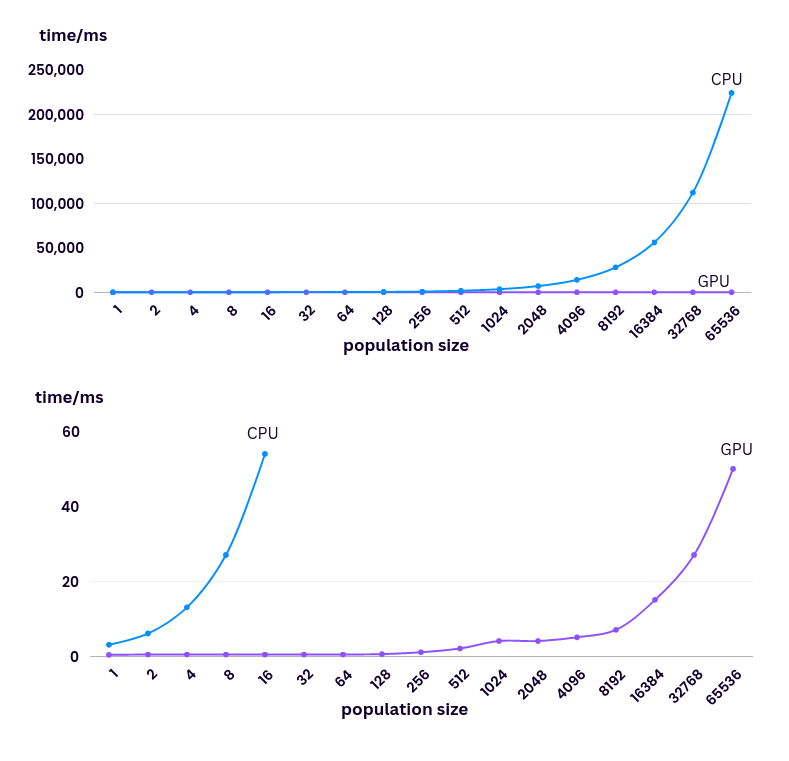
\includegraphics[width=3in]{popsizetime.png}
\caption{3D cube in x, y, z axis}
\label{fig:my_label}
GPU vs CPU time per 1 episode step for different population sizes. GPU is running a program written in GLSL and CPU in Python. It can be seen that the CPU time grows much more quickly.


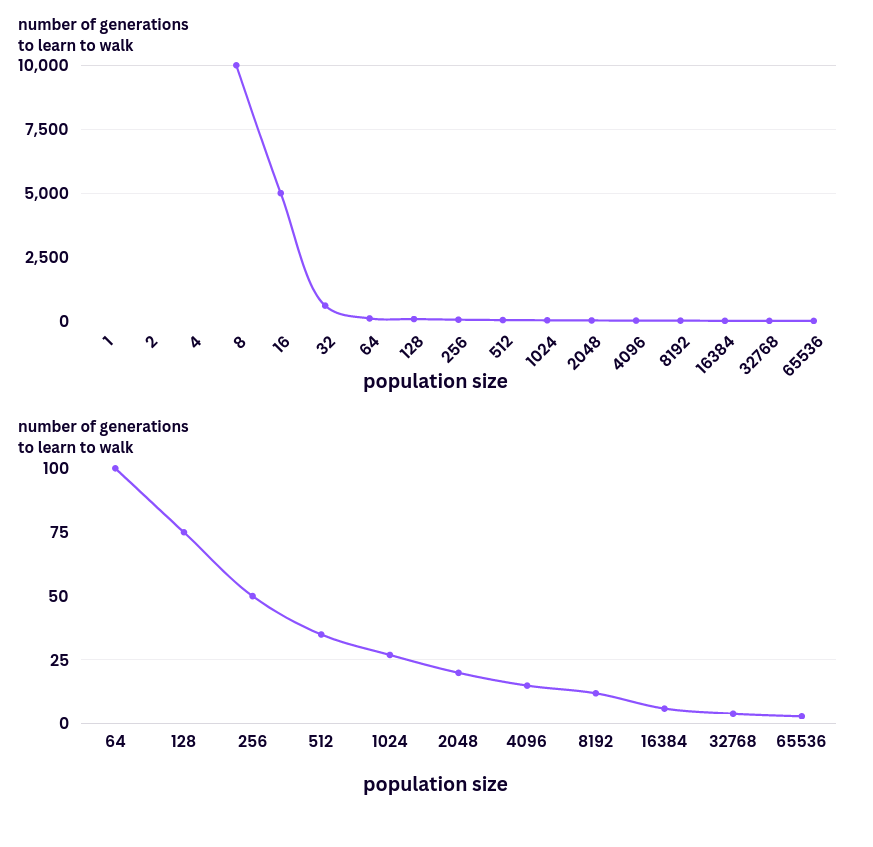
\includegraphics[width=3in]{numberofgenerationstolearntowalk.png}
As the population size grows number of generations to learn to walk falls. This is because when the population size is large, the probability that any creature is walking by pure chance is high.

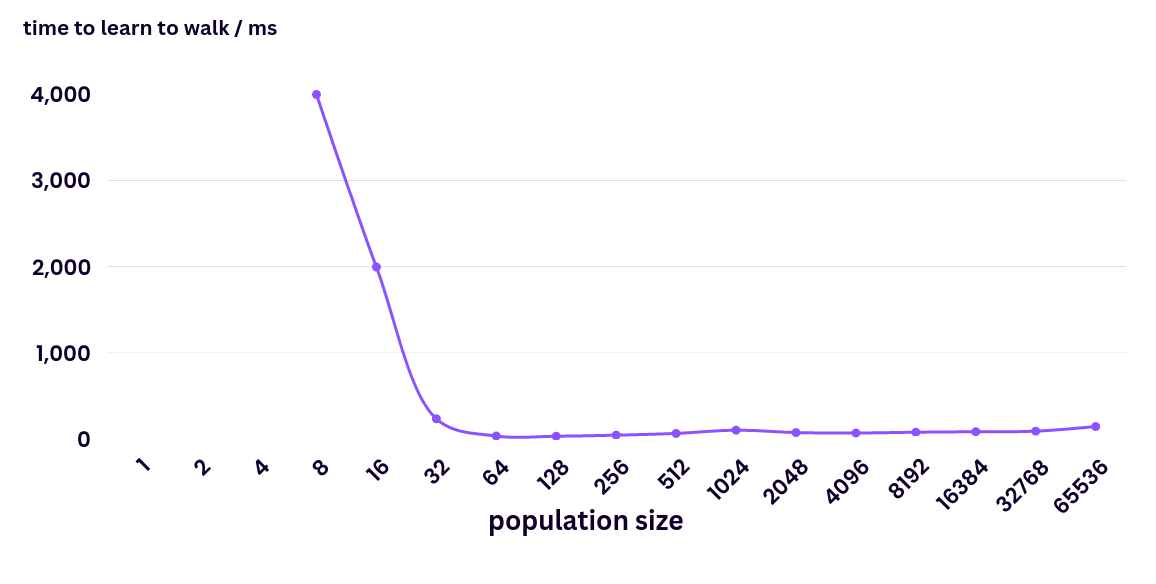
\includegraphics[width=3in]{resources/timetolearntowalk.png}
Illustration of advantage of using GPU's to simulate physics and run creature learning.

#if 0
\begin{figure}[H]
    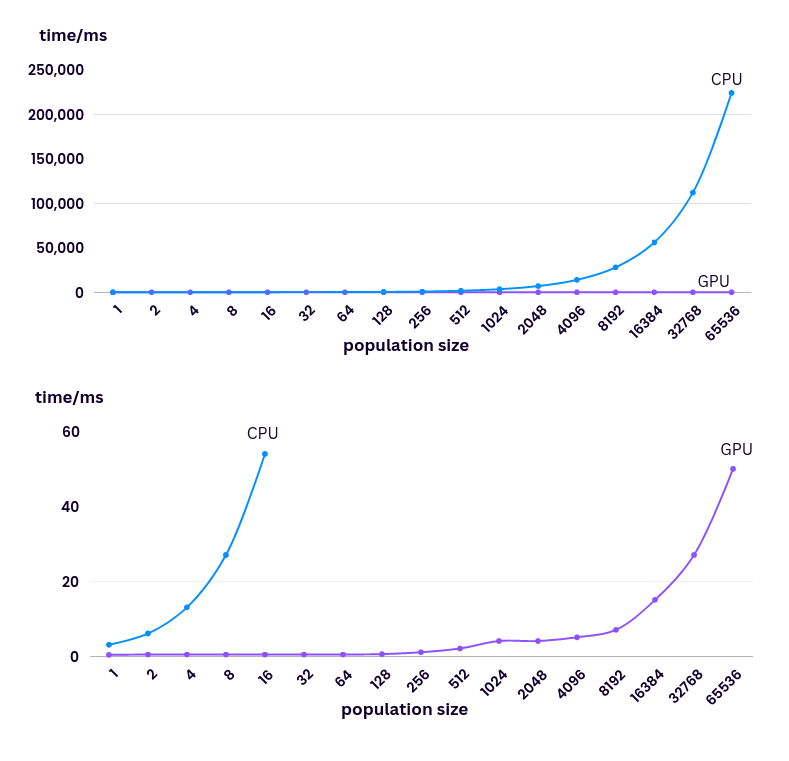
\includegraphics[width=3in]{popsizetime.png} %veličina u odnosu na širinu linije
    \caption{GPU vs CPU time per 1 episode step for different population sizes. GPU is running a program written in GLSL and CPU in Python. It can be seen that the CPU time grows much more quickly.}
    \label{fig:struktura} %label mora biti drugaciji za svaku sliku
\end{figure}

\begin{figure}[H]
    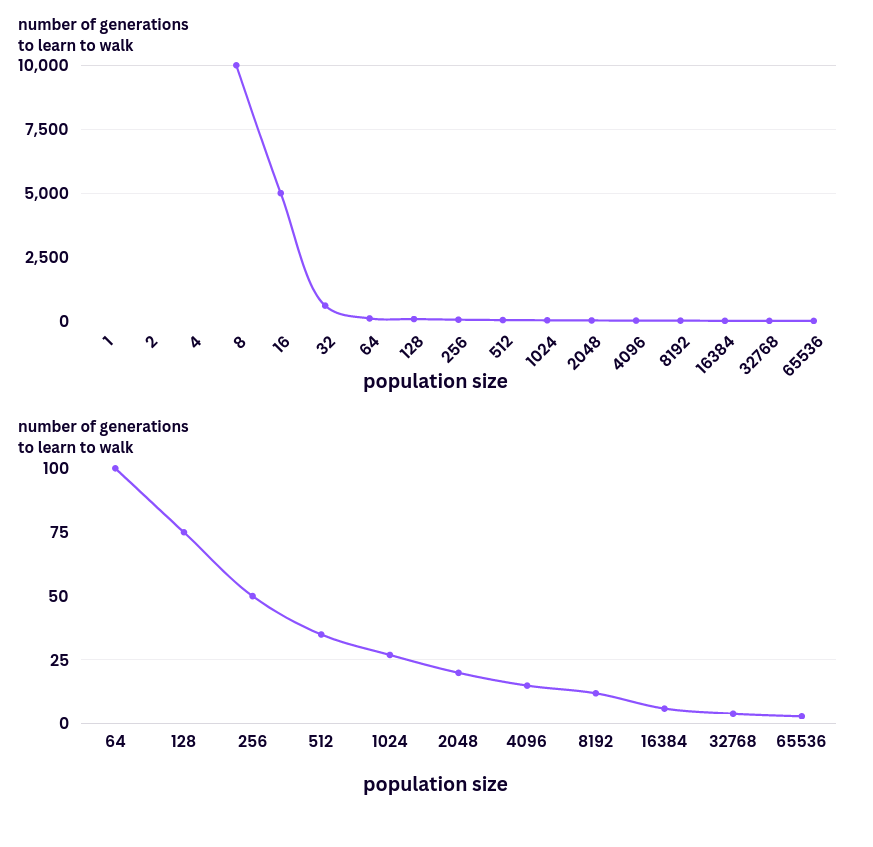
\includegraphics[width=3in]{numberofgenerationstolearntowalk.png} %veličina u odnosu na širinu linije
    \caption{As the population size grows number of generations to learn to walk falls. This is because when the population size is large, the probability that any creature is walking by pure chance is high.}
    \label{fig:struktura} %label mora biti drugaciji za svaku sliku
\end{figure}

\begin{figure}[H]
    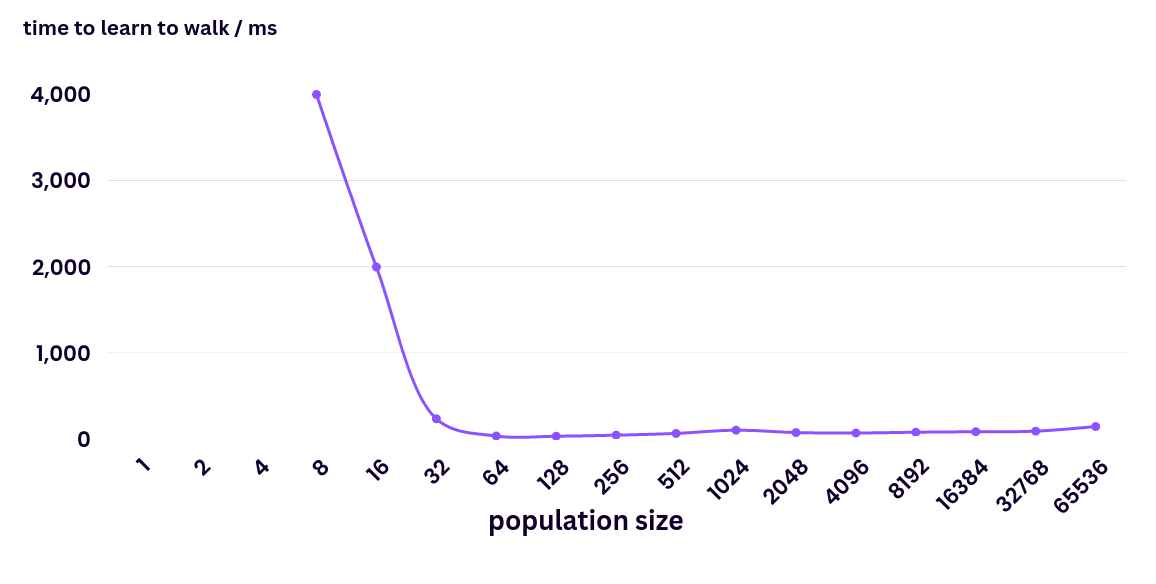
\includegraphics[width=3in]{resources/timetolearntowalk.png} %veličina u odnosu na širinu linije
    \caption{Illustration of advantage of using GPU's to simulate physics and run creature learning.}
    \label{fig:struktura} %label mora biti drugaciji za svaku sliku
\end{figure}
#endif

\section{\huge Conclusion}

    In conclusion, this project has successfully implemented a system for visualizing and simulating the movement of shapes using shaders and buffers. Our study has shown that increasing the number of instances in a neural network can result in a faster learning process for the task of simulating walking. However, it also leads to slower computing speeds and longer iteration times. Thus, it is important to strike a balance between the number of instances and the speed of computing in order to optimize the performance of the neural network. Further research can be conducted to identify the optimal number of instances for different types of tasks and computing environments.

\subsection{\LARGE Future work}

    There is still room for improvement in the future. One area for improvement is the physics simulation, which could be optimized to run more efficiently. Another potential improvement is the use of more advanced algorithms for matrix multiplication, such as the Winograd algorithm, which has a lower computational complexity compared to naive matrix multiplication. Additionally, the size of the neural networks used in the genetic computation could be reduced as they are not required to be complex in this project, this will speed up the process and make it more efficient.


\bibliographystyle{IEEEtran}
\bibliography{refs}

\end{document}
